\usetikzlibrary{arrows.meta,decorations.pathmorphing}

\begin{frame}{`forwarding' exception as signal}
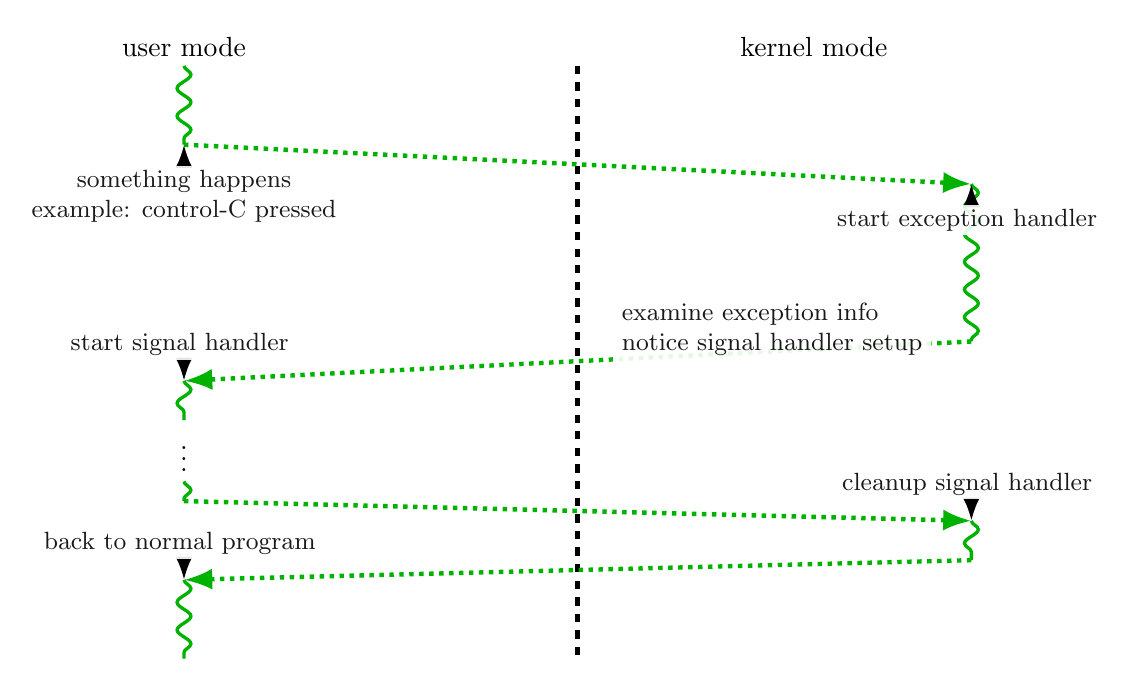
\begin{tikzpicture}
\draw[ultra thick,dashed] (1, -.5) -- (1, -8);
\begin{scope}[every node/.style={anchor=south,align=center}]
    \node at (-4, -.5) {user mode};
    \node at (4, -.5) {kernel mode};
\end{scope}
\tikzset{
    snake/.style={very thick,decorate,decoration={snake}},
    >=Latex,
    process A/.style={green!70!black},
    OS code/.style={blue!70!black},
},
\draw[snake,process A] (-4, -.5) -- (-4, -1.5) coordinate (before enter kernel);
\draw[snake,process A] (6, -2) coordinate (after enter kernel) -- (6, -4) coordinate (before run sighandler);
\draw[snake,process A] (-4, -4.5) coordinate (run sighandler) -- (-4, -5) coordinate (after run sighandler);
\node[anchor=north] (sighandler dots) at (after run sighandler) {\vdots};
\draw[snake,process A](sighandler dots.south) -- ++(0, -.25) coordinate (sighandler ret);
\draw[snake,process A] ([xshift=10cm,yshift=-.25cm]sighandler ret) coordinate (sighandler ret kern)
    --  ++(0cm, -.5cm) coordinate (end sighandler ret kern);
\draw[snake,process A] ([xshift=-10cm,yshift=-.25cm]end sighandler ret kern) 
    coordinate (post sighandler) -- ++(0, -1);
\draw[process A,ultra thick,->,dotted] (before enter kernel) -- (after enter kernel);
\draw[process A,ultra thick,->,dotted] (before run sighandler) -- (run sighandler);
\draw[process A,ultra thick,->,dotted] (sighandler ret) -- (sighandler ret kern);
\draw[process A,ultra thick,->,dotted] (end sighandler ret kern) -- (post sighandler);
\node[align=left,font=\small,fill=white,fill opacity=0.9,anchor=south east] 
    at ([xshift=-.5cm,yshift=-.3cm]before run sighandler) {
    examine exception info \\
    notice signal handler setup
};
\draw[dotted,very thick,<-] (before enter kernel) -- ++(0cm, -.25cm) node[below,align=center,font=\small,fill=white,fill opacity=0.9, inner sep=0.5mm] {
    something happens \\
    example: control-C pressed
};
\draw[dotted, very thick,<-] (after enter kernel) -- ++(0cm, -.25cm) node[below,align=center, font=\small,fill=white,fill opacity=0.9,inner sep=0.5mm] {
    start exception handler
};
\draw[dotted,very thick,<-] (run sighandler) -- ++(0cm, .25cm) node[above,align=center,font=\small,fill=white,fill opacity=0.9, inner sep=0.5mm] {
    start signal handler
};
\draw[dotted,very thick,<-] (sighandler ret kern) -- ++(0cm, .25cm) node[above,align=center,font=\small,fill=white,fill opacity=0.9, inner sep=0.5mm] {
    cleanup signal handler
};
\draw[dotted,very thick,<-] (post sighandler) -- ++(0cm, .25cm) node[above,align=center,font=\small,fill=white,fill opacity=0.9, inner sep=0.5mm] {
    back to normal program
};
%\draw[process A,ultra thick,->,dotted] (before exit kernel) -- (after exit kernel);
%\draw[dotted,very thick,<-] (before exit kernel) -- ++(0cm, -.25cm) node[below,font=\small,fill=white,fill opacity=0.9, inner sep=0.5mm,align=center] {};
\end{tikzpicture}
\end{frame}

